\documentclass[a4paper, titlepage]{article}
\usepackage[round, sort, numbers]{natbib}
\usepackage[utf8]{inputenc}
\usepackage{amsfonts, amsmath, amssymb, amsthm}
\usepackage{color}
\usepackage{listings}
\usepackage{marvosym}
\usepackage{mathtools}
\usepackage{paralist}
\usepackage{parskip}
\usepackage{subfig}
\usepackage{tikz}
\usepackage{titlesec}

\numberwithin{figure}{section}
\numberwithin{table}{section}

\usetikzlibrary{arrows, automata, backgrounds, petri, positioning}
\tikzstyle{place}=[circle, draw=blue!50, fill=blue!20, thick]
\tikzstyle{transition}=[rectangle, draw=black!50, fill=black!20, thick]

% define new commands for sets and tuple
\newcommand{\setof}[1]{\ensuremath{\left \{ #1 \right \}}}
\newcommand{\tuple}[1]{\ensuremath{\left \langle #1 \right \rangle }}
\newcommand{\card}[1]{\ensuremath{\left \vert #1 \right \vert }}

\makeatletter
\newcommand\objective[1]{\def\@objective{#1}}
\newcommand{\makecustomtitle}{%
	\begin{center}
		\huge\@title \\
		[1ex]\small Aurélien Coet, Dimitri Racordon
	\end{center}
	\@objective
}
\makeatother

\begin{document}

\title{Outils formels de Modélisation \\ 2\textsuperscript{ème} séance d'exercices}
\author{Aurélien Coet, Dimitri Racordon}
\objective{Dans cette séance d'exercices, nous allons aborder de manière intuitive les réseaux de Petri, par le biais de l'observation et de la création de modèles simples.}

\makecustomtitle

\section{Transformations 101 ($\bigstar$)}

Réécrivez les réseaux de Petri suivants en automates à états finis, tout en imitant au mieux leurs comportements respectifs.

\begin{figure}[ht]
  \centering
  \begin{tabular}{cc}
  \subfloat[]{%
  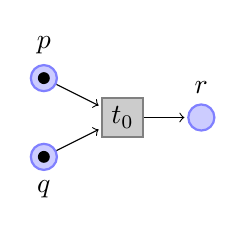
\begin{tikzpicture}
      \node[place,tokens=1] (p) [label=above:$p$] {};
	   \node[place,tokens=1] (q) [below of=p, label=below:$q$] {};
	   \node[place] (r) [right of=p, xshift=1cm, yshift=-0.5cm, label=above:$r$] {};
      \node [transition] (t0) [right of=p, yshift=-0.5cm] {$t_0$}
	   edge [pre] (p)
      edge [pre] (q)
	   edge [post] (r);
  \end{tikzpicture}
  } &
  \subfloat[]{%
  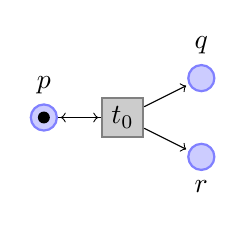
\begin{tikzpicture}
      \node[place,tokens=1] (p) [label=above:$p$] {};
      \node[place] (q) [right of=p, xshift=1cm, yshift=0.5cm, label=above:$q$] {};
	   \node[place] (r) [right of=p, xshift=1cm, yshift=-0.5cm, label=below:$r$] {};
      \node [transition] (t0) [right of=p] {$t_0$}
	   edge [pre] (p)
      edge [post] (p)
      edge [post] (q)
	   edge [post] (r);
  \end{tikzpicture}
  } \\
  \multicolumn{2}{c}{\subfloat[]{%
  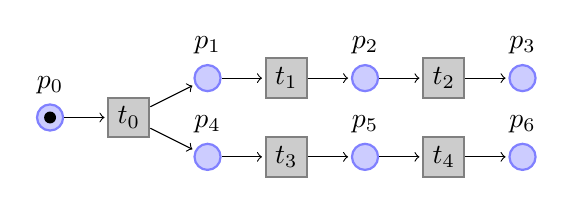
\begin{tikzpicture}
      \node[place,tokens=1] (p0) [label=above:$p_0$] {};
	   \node[place] (p1) [right of=p0, xshift=1cm, yshift=0.5cm, label=above:$p_1$] {};
	   \node[place] (p2) [right of=p1, xshift=1cm, label=above:$p_2$] {};
	   \node[place] (p3) [right of=p2, xshift=1cm, label=above:$p_3$] {};

	   \node[place] (p4) [right of=p0, xshift=1cm, yshift=-0.5cm, label=above:$p_4$] {};
	   \node[place] (p5) [right of=p4, xshift=1cm, label=above:$p_5$] {};
	   \node[place] (p6) [right of=p5, xshift=1cm, label=above:$p_6$] {};

      \node [transition] (t0) [right of=p0] {$t_0$}
	   edge [pre] (p0)
      edge [post] (p1)
	   edge [post] (p4);
      \node [transition] (t1) [right of=p1] {$t_1$}
	   edge [pre] (p1) edge [post] (p2);
      \node [transition] (t2) [right of=p2] {$t_2$}
	   edge [pre] (p2) edge [post] (p3);
      \node [transition] (t3) [right of=p4] {$t_3$}
	   edge [pre] (p4) edge [post] (p5);
      \node [transition] (t4) [right of=p5] {$t_4$}
      edge [pre] (p5) edge [post] (p6);
  \end{tikzpicture}
}}
\end{tabular}
\end{figure}

Est-il possible de réécrire n'importe quel réseau de Petri en automate à états finis? Justifiez votre réponse.

\section{Non déterminisme ($\bigstar$$\bigstar$)}

Considérez le réseau de Petri de la figure \ref{fig:exclusion}.

\begin{enumerate}
\item De quel type d'algorithme ce réseau représente-t-il le comportement?
\item A partir du marquage initial, existe-t-il un marquage pour lequel à la fois $t_1$ et $t_2$ sont tirables?
\item Indiquez un état possible du réseau après 50 tirs de transitions?
\item Après 50 tirs de transitions, combien de fois $t_0$ aura-t-elle été tirable?
\end{enumerate}

\begin{figure}[ht]
\centering
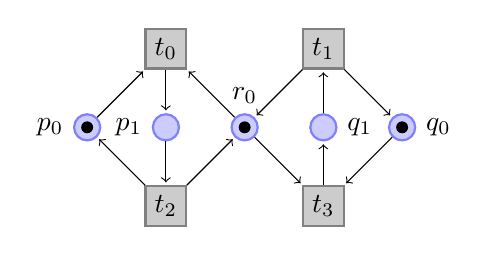
\begin{tikzpicture}
    \node[place,tokens=1] (p0) [label=left:$p_0$] {};
    \node[place] (p1) [right of=p0, label=left:$p_1$] {};
    \node[place,tokens=1] (r0) [right of=p1, label=above:$r_0$] {};
    \node[place] (q1) [right of=r0, label=right:$q_1$] {};
    \node[place,tokens=1] (q0) [right of=q1, label=right:$q_0$] {};

    \node [transition] (t0) [above of=p1] {$t_0$}
    edge [pre] (p0) edge [pre] (r0)
	edge [post] (p1);
    \node [transition] (t1) [above of=q1] {$t_1$}
	edge [pre] (q1)
	edge [post] (r0) edge [post] (q0);
    \node [transition] (t2) [below of=p1] {$t_2$}
	  edge [pre] (p1)
    edge [post] (r0) edge [post] (p0);
    \node [transition] (t3) [below of=q1] {$t_3$}
	  edge [pre] (q0) edge [pre] (r0)
	edge [post] (q1);
\end{tikzpicture}
\caption{Un réseau de Petri non déterministe}
\label{fig:exclusion}
\end{figure}

\newpage
\section{Circulation [\Keyboard] ($\bigstar$$\bigstar$$\bigstar$)}

Le réseau de la figure \ref{fig:light} est une ébauche représentant un feu de circulation, dont le comportement est défini par la séquence $(r) \rightarrow (g) \rightarrow (y) \rightarrow (r) \dots$ Complétez l'ébauche afin de relever le nombre de fois que le feu \emph{passe} au orange.

\begin{figure}[ht]
\centering
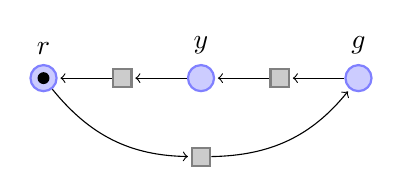
\begin{tikzpicture}[bend angle=25]
    \node[place,tokens=1] (r) [label=90:$r$] {};
	\node[place] (y) [right of=r, xshift=1cm, label=90:$y$] {};
	\node[place] (g) [right of=y, xshift=1cm, label=90:$g$] {};

    \node [transition] (t0) [below of=y] {}
	  edge [pre, bend left] (r) edge [post, bend right] (g);
    \node [transition] (t1) [right of=y] {}
	edge [pre] (g) edge [post] (y);
    \node [transition] (t2) [right of=r] {}
	edge [pre] (y) edge [post] (r);
\end{tikzpicture}
\caption{Un feu de circulation}
\label{fig:light}
\end{figure}

Un feu de circulation suisse ne suit pas la séquence décrite ci-dessus, mais plutôt $(r) \rightarrow (r) \land (y) \rightarrow (g) \rightarrow (y) \rightarrow (r) \dots$.
Modifiez le réseau afin de garantir que seul ce comportement peut être représenté par le réseau.

Vous trouverez dans le dossier \texttt{Exercise/} de ce dépôt un projet F\# contenant une implémentation du modèle de feu de circulation présenté dans cet exercice. 
Modifiez le code dans le fichier \texttt{Program.fs} pour refléter les transformations apportées au modèle dans les points précédents. 

\end{document}
